\section{Baselines and Results}
\label{sec:results}

This section reports the reference baselines that ship with \wcabench. The
numbers below are the \emph{actual} outputs of the released baselines on the
official export; they are taken directly from the repository's leaderboard and
multi-seed artifacts and are not illustrative. We emphasize two honest caveats
before presenting them. First, these results were produced in the benchmark's
\emph{small} mode, which samples test competitions and a representative
training subset so that the full baseline suite runs on a single machine; the
definitive leaderboard must be recomputed on the full data under the
rolling-window protocol. Second, because the benchmark's goal is to define a
question rather than to win it, the value of these numbers lies in their
comparability, not in their absolute magnitude. The hardware used is documented
in Section~\ref{sec:compute}.

\subsection{Baseline coverage}
\label{sec:results-taxonomy}

The released suite contains \textbf{21 baselines} spanning \textbf{six
methodological families}---statistical, tree, deep, graph, Bayesian and
causal---plus a set of domain and trivial reference models, with at least four
baselines for every task. Table~\ref{tab:coverage} maps the families onto the
tasks. \emph{Trivial} baselines establish a lower bound (historical mean,
historical rate). \emph{Domain} baselines encode current practice (the \wca{}
psychology sheet, the historical \DNF{} rate, kernel-density models).
\emph{Methodological} baselines test whether additional
machinery---boosting, sequence models, graph propagation, Bayesian shrinkage or
causal identification---actually helps. All heavy baselines now run on their
native backends: the tree models use real XGBoost and the GNN uses its native
CUDA path (Section~\ref{sec:compute}).

\begin{table}[t]
  \centering
  \small
  \begin{threeparttable}
  \caption{Baseline coverage: 21 baselines across six methodological families
  plus domain/trivial references.}
  \label{tab:coverage}
  \begin{tabular}{@{}p{2.4cm}p{8.2cm}p{2.6cm}@{}}
    \toprule
    Family & Baselines & Tasks \\
    \midrule
    Domain / trivial & \texttt{history\_mean}, \texttt{kde}, \texttt{psych\_sheet},
                       \texttt{historical\_dnf\_rate} & T1, T2, T3 \\
    Statistical & \texttt{ridge\_log}, \texttt{logistic}, \texttt{kde\_simulation},
                  \texttt{plackett\_luce}, \texttt{spearman\_correlation},
                  \texttt{exponential\_decay}, \texttt{changepoint}, \texttt{gp\_evt} & T1--T5 \\
    Tree & \texttt{xgboost\_log}, \texttt{xgboost\_dnf} & T1, T3 \\
    Deep & \texttt{lstm} & T1 \\
    Graph & \texttt{gnn} & T2 \\
    Bayesian & \texttt{beta\_binomial}, \texttt{hierarchical\_shrinkage} & T3, T4 \\
    Causal & \texttt{did\_proxy}, \texttt{iv\_2sls}, \texttt{causal\_forest} & T5 \\
    \bottomrule
  \end{tabular}
  \end{threeparttable}
\end{table}

\subsection{Main results}
\label{sec:results-main}

Table~\ref{tab:main} reports every baseline with its primary metric for the
seed-42 run and the number of evaluated instances. The best value per task is
in bold.

\begin{table}[t]
  \centering
  \small
  \begin{threeparttable}
  \caption{All 21 reference baselines (sampled test set, official export
  v2.0.2, seed 42, GPU run). Primary metrics are in the ``best'' direction
  indicated; $n$ is the number of evaluated instances. All values are measured,
  not hypothetical.}
  \label{tab:main}
  \begin{tabular}{@{}llllr@{}}
    \toprule
    Task & Baseline & Family & Primary metric & Value ($n$) \\
    \midrule
    \multirow{5}{*}{\task{1} Result}
      & \texttt{xgboost\_log} & tree & \maelog{} \arrdown & \textbf{0.1639} (2196) \\
      & \texttt{history\_mean} & trivial & \maelog{} \arrdown & 0.6657 (2196) \\
      & \texttt{kde} & domain & \maelog{} \arrdown & 0.6657 (2196) \\
      & \texttt{ridge\_log} & statistical & \maelog{} \arrdown & 1.0068 (2196) \\
      & \texttt{lstm} & deep & \maelog{} \arrdown & 1.0440 (2196) \\
    \midrule
    \multirow{4}{*}{\task{2} Placement}
      & \texttt{plackett\_luce} & statistical & Kendall $\kendall$ \arrup & \textbf{0.7673} (2260) \\
      & \texttt{kde\_simulation} & statistical & Kendall $\kendall$ \arrup & \textbf{0.7673} (2260) \\
      & \texttt{psych\_sheet} & domain & Kendall $\kendall$ \arrup & \textbf{0.7673} (2260) \\
      & \texttt{gnn} & graph & Kendall $\kendall$ \arrup & 0.5670 (2260) \\
    \midrule
    \multirow{4}{*}{\task{3} DNF}
      & \texttt{xgboost\_dnf} & tree & \aucpr{} \arrup & \textbf{0.3731} (2260) \\
      & \texttt{beta\_binomial} & Bayesian & \aucpr{} \arrup & 0.3725 (2260) \\
      & \texttt{historical\_dnf\_rate} & domain & \aucpr{} \arrup & 0.3591 (2260) \\
      & \texttt{logistic} & statistical & \aucpr{} \arrup & 0.2290 (2260) \\
    \midrule
    \multirow{4}{*}{\task{4} Limit}
      & \texttt{gp\_evt} & statistical & LOO stability \arrdown & \textbf{0.9836} (21 events) \\
      & \texttt{exponential\_decay} & statistical & LOO stability \arrdown & 6{,}485{,}301 (21 events) \\
      & \texttt{hierarchical\_shrinkage} & Bayesian & LOO stability \arrdown & 9{,}260{,}100 (21 events) \\
      & \texttt{changepoint} & statistical & LOO stability \arrdown & n/r \\
    \midrule
    \multirow{4}{*}{\task{5} Transfer}
      & \texttt{spearman\_correlation} & statistical & identified pairs \arrup & \textbf{413} (80{,}000) \\
      & \texttt{causal\_forest} & causal & identified pairs \arrup & 312 (80{,}000) \\
      & \texttt{iv\_2sls} & causal & identified pairs \arrup & 270 (80{,}000) \\
      & \texttt{did\_proxy} & causal & identified pairs \arrup & 6 (80{,}000) \\
    \bottomrule
  \end{tabular}
  \begin{tablenotes}\footnotesize
    \item ``n/r'' = not reported: the change-point baseline does not emit a
          leave-one-out stability statistic. The \task{4} stability figures are
          dominated by multi-blind event pairs whose limit scale is extremely
          large; Appendix~\ref{app:limit} gives a scale-robust, per-event view.
  \end{tablenotes}
  \end{threeparttable}
\end{table}

\subsection{Multi-seed evaluation}
\label{sec:results-multiseed}

Because the seed controls how test competitions and the training subset are
resampled, repeating a run over several seeds measures the \emph{evaluation-set
sampling variance} of each metric---exactly the uncertainty a single run cannot
reveal. Table~\ref{tab:multiseed} reports the mean $\pm$ standard deviation
over seeds $\{42,43,44\}$ for every baseline. For \task{4} and \task{5} the
deterministic estimators are seed-invariant (std $=0$), so only \task{1},
\task{2} and \task{3} show meaningful spread.

\begin{table}[t]
  \centering
  \small
  \begin{threeparttable}
  \caption{Multi-seed results over seeds $\{42,43,44\}$ (small mode, GPU).
  Values are mean $\pm$ standard deviation of the primary metric; the seed
  resamples the evaluation set, so the spread reflects evaluation-set sampling
  variance. Best mean per task in bold.}
  \label{tab:multiseed}
  \begin{tabular}{@{}llll@{}}
    \toprule
    Task & Baseline & Metric & Mean $\pm$ std \\
    \midrule
    \multirow{5}{*}{\task{1} Result}
      & \texttt{xgboost\_log} & \maelog{} & \textbf{0.1055 $\pm$ 0.0417} \\
      & \texttt{history\_mean} & \maelog{} & 0.4003 $\pm$ 0.1945 \\
      & \texttt{kde} & \maelog{} & 0.4003 $\pm$ 0.1945 \\
      & \texttt{ridge\_log} & \maelog{} & 0.9381 $\pm$ 0.0526 \\
      & \texttt{lstm} & \maelog{} & 0.9436 $\pm$ 0.0754 \\
    \midrule
    \multirow{4}{*}{\task{2} Placement}
      & \texttt{psych\_sheet} & Kendall $\kendall$ & \textbf{0.8132 $\pm$ 0.0342} \\
      & \texttt{plackett\_luce} & Kendall $\kendall$ & 0.8132 $\pm$ 0.0342 \\
      & \texttt{kde\_simulation} & Kendall $\kendall$ & 0.8132 $\pm$ 0.0342 \\
      & \texttt{gnn} & Kendall $\kendall$ & 0.7440 $\pm$ 0.1258 \\
    \midrule
    \multirow{4}{*}{\task{3} DNF}
      & \texttt{beta\_binomial} & \aucpr{} & \textbf{0.2938 $\pm$ 0.0570} \\
      & \texttt{xgboost\_dnf} & \aucpr{} & 0.2779 $\pm$ 0.0724 \\
      & \texttt{historical\_dnf\_rate} & \aucpr{} & 0.2631 $\pm$ 0.0690 \\
      & \texttt{logistic} & \aucpr{} & 0.1687 $\pm$ 0.0429 \\
    \midrule
    \multirow{3}{*}{\task{4} Limit}
      & \texttt{gp\_evt} & LOO stability & \textbf{0.9836 $\pm$ 0.0000} \\
      & \texttt{exponential\_decay} & LOO stability & 6{,}485{,}301 $\pm$ 0 \\
      & \texttt{hierarchical\_shrinkage} & LOO stability & 9{,}260{,}100 $\pm$ 0 \\
    \midrule
    \multirow{4}{*}{\task{5} Transfer}
      & \texttt{spearman\_correlation} & pairs & \textbf{413 $\pm$ 0} \\
      & \texttt{causal\_forest} & pairs & 312 $\pm$ 0 \\
      & \texttt{iv\_2sls} & pairs & 270 $\pm$ 0 \\
      & \texttt{did\_proxy} & pairs & 2 $\pm$ 0 \\
    \bottomrule
  \end{tabular}
  \end{threeparttable}
\end{table}

The multi-seed view is informative in three ways. \task{1} is the most
seed-sensitive task: the tree model averages $0.1055\pm0.0417$ while the LSTM
averages $0.9436\pm0.0754$, roughly nine times worse in the mean and with a
comparable relative spread, so the deep/graph deficit is not an artifact of one
split. \task{3} changes its ranking: the Beta--Binomial model is best on
average ($0.2938\pm0.0570$) whereas the tree model is first in the single
seed-42 run ($0.3731$ vs $0.3725$)---the two are within one standard deviation
of each other, which is itself the honest conclusion and the reason a single
run should not be over-interpreted. For \task{2}, the domain and statistical
rankings are again indistinguishable on average ($0.8132\pm0.0342$) while the
GNN is clearly lower ($0.7440\pm0.1258$).

\subsection{\task{1}: result prediction}
\label{sec:results-t1}

Tree-based regression on log-transformed targets is the strongest \task{1}
baseline, with \maelog{} $=0.1639$ on $n=2196$ instances (and
$0.1055\pm0.0417$ across seeds). Replacing it with a competitor's historical
mean (\texttt{history\_mean}) or a kernel density estimate (\texttt{kde})
roughly quadruples the error to $0.6657$. A naive log-linear ridge model
reaches $1.0068$, and---strikingly---a sequence model (\texttt{lstm}) is the
\emph{worst} baseline at $1.0440$ ($0.9436\pm0.0754$ across seeds), worse even
than the historical mean. The ordering is intuitive once stated: results are
highly autocorrelated within a competitor, so a flexible model that exploits
recent history and event context wins, whereas a global linear extrapolation or
a lightly-tuned recurrent model is badly misspecified across the wildly
different event scales. That a deep sequence model fails to beat a trivial
baseline is itself a useful benchmark result.

The advantage of the tree model is not uniform. Its secondary metric is
\rmselog{} $=0.4490$, noticeably larger than the mean error, indicating a tail
of hard predictions (for example sparse blindfolded events) that dominate
squared loss. This is exactly why stratified reporting matters, as shown below.

\subsection{\task{2}: placement prediction}
\label{sec:results-t2}

The headline observation for \task{2} is a three-way tie. The official \wca{}
psychology sheet, a Plackett--Luce model and a kernel-density Monte Carlo
simulation all achieve Kendall $\kendall=0.7673$ to four decimal places on the
same $n=2260$ rounds (and $0.8132\pm0.0342$ across seeds); the psychology
sheet's top-3 overlap is $0.7595$. Their paired differences are exactly zero,
so no significance test is defined. At this sample size, additional
distributional modelling buys nothing over a good point ranking.

The graph baseline tells the opposite story for a different family: the GNN
reaches only $\kendall=0.5670$ with a top-3 overlap of $0.5021$ (multi-seed
$0.7440\pm0.1258$), substantially below every simple ranking model. The paired
comparison against the psychology sheet gives $\Delta=0.200$
(95\% CI $[0.122,0.268]$), $p=3.2\times10^{-7}$ and a medium effect size
(Cohen's $d=0.56$, Cliff's $\delta=0.30$). This is a genuinely useful negative
result: it tells the community where effort is \emph{not} currently rewarded,
and it sets a strong domain baseline that any new ranking method must beat to
be interesting.

\subsection{\task{3}: DNF prediction}
\label{sec:results-t3}

The tree-based classifier attains \aucpr{} $=0.3731$ (\aucroc{} $=0.5911$,
F1 $=0.2121$, MCC $=0.3148$, calibration error $=0.1584$), narrowly ahead of a
Bayesian Beta-Binomial posterior (\aucpr{} $=0.3725$) and the historical-rate
prior ($0.3591$); a logistic model trails badly at $0.2290$. Crucially, the gap
between the tree model and the historical prior is \emph{not} statistically
significant---$\Delta=0.0005$ (95\% CI $[-0.003,0.003]$), $p=0.749$, negligible
effect ($d=0.002$)---and the tree model's paper-thin edge over the
Beta--Binomial prior is significant but small ($\Delta=0.042$,
$p=4.5\times10^{-7}$, $d=0.16$), while Beta--Binomial is in fact best on
average across seeds (Table~\ref{tab:multiseed}). The logistic deficit is large
and highly significant ($\Delta=0.278$, $p=1.6\times10^{-15}$, $d=1.57$).

This reinforces the task's design lesson: under rarity and imbalance, a strong,
well-calibrated prior is hard to beat, and \aucroc{} alone is misleading. The
evaluated test set has a positive rate of $18.27\%$, far above the $3.18\%$
global attempt-level \DNF{} rate, because the task conditions on rounds that
reach the decision point. Even so, the event-level breakdown is extreme: the
three-by-three blindfolded subset has a $94.5\%$ positive rate, while several
speed-solving events have single-digit rates. Any unstratified average would be
misleading.

\subsection{\task{4}: human-limit estimation}
\label{sec:results-t4}

Human-limit estimation has no observable ground truth, so the benchmark reports
stability rather than accuracy. The Gaussian-process plus extreme-value
baseline (\texttt{gp\_evt}) is by far the most stable, with an aggregate
leave-one-out stability of $0.9836$, two orders of magnitude smaller than the
exponential-decay model ($6{,}485{,}301$) and the Bayesian hierarchical
shrinkage model ($9{,}260{,}100$)---both of which are inflated by the
multi-blind event, whose encoded limit is of order $10^8$. The change-point
baseline refuses to emit a stability statistic and is scored ``n/r''. All three
stability aggregates have very wide confidence intervals and are not
significantly separated at $21$ events ($p\ge0.30$), which we report rather than
oversell.

Point estimates differ in ways that matter for domain use. For three-by-three,
\texttt{gp\_evt} gives $329.38$ centiseconds ($3.29$~s, convergence 2028),
the change-point model $302.25$ centiseconds ($3.02$~s), and exponential decay
$373.69$ centiseconds ($3.74$~s). All lie well above the commonly cited domain
anchor of $\approx 2.37$~seconds---a discrepancy we treat as the expected
signature of extrapolation risk rather than as a bug.

\subsection{\task{5}: skill transfer}
\label{sec:results-t5}

The correlational baseline marks $413$ event pairs as ``identifiable'' out of
$17 \times 17$ ordered pairs. As identification assumptions tighten, the count
falls monotonically: causal forest $312$, instrumental variables (2SLS) $270$,
and difference-in-differences only $6$ (multi-seed $2$), all on the same
$80{,}000$-competitor sample. Every causal estimator differs from the
correlational baseline with $p\le5\times10^{-21}$, with effect sizes ranging
from medium to huge (Cliff's $\delta=0.19$ for the causal forest, $0.29$ for
IV, and $0.91$ for DID). The gap quantifies how much naive correlation
over-claims: it cannot separate genuine transfer from shared talent and
training effort, and the stricter methods identify fewer and fewer pairs.

None of these estimators is causal ground truth---DID relies on parallel
trends, IV on instrument exogeneity, and causal forests on unconfoundedness---so
the benchmark's contribution is not a single number but the \emph{spread}
across assumptions. Reporting the count of identifiable pairs, rather than
forcing an estimate for every cell, is a deliberate design choice that makes
non-identifiability visible.

\subsection{Statistical significance}
\label{sec:results-significance}

Table~\ref{tab:significance} collects the key paired comparisons from the
released reports. All tests use the same paired unit (competition $\times$ event
$\times$ round, or event for \task{4}), the same seed (42) and a $1000$-resample
bootstrap for the confidence intervals, following Section~\ref{sec:protocol}.

\begin{table}[t]
  \centering
  \small
  \begin{threeparttable}
  \caption{Key paired comparisons against each task's reference baseline.
  For \task{1} and \task{4} lower is better, so a positive $\Delta$ means the
  model is \emph{worse}; for \task{2} and \task{3} higher is better. Effect
  sizes are Cohen's $d$.}
  \label{tab:significance}
  \begin{tabular}{@{}llrrr@{}}
    \toprule
    Task & Comparison (vs reference) & $\Delta$ & 95\% CI & $p$ \\
    \midrule
    \task{1} & \texttt{lstm} vs \texttt{xgboost\_log} & $+1.087$ & $[0.810,1.509]$ & $5.2\mathrm{e}{-8}$ \\
    \task{1} & \texttt{ridge\_log} vs \texttt{xgboost\_log} & $+0.906$ & $[0.723,1.119]$ & $3.2\mathrm{e}{-14}$ \\
    \task{1} & \texttt{history\_mean} vs \texttt{xgboost\_log} & $+0.685$ & $[0.305,1.089]$ & $6.5\mathrm{e}{-4}$ \\
    \task{2} & \texttt{gnn} vs \texttt{psych\_sheet} & $+0.200$ & $[0.122,0.268]$ & $3.2\mathrm{e}{-7}$ \\
    \task{3} & \texttt{historical\_dnf\_rate} vs \texttt{xgboost\_dnf} & $+0.0005$ & $[-0.003,0.003]$ & $0.749$ \\
    \task{3} & \texttt{beta\_binomial} vs \texttt{xgboost\_dnf} & $+0.042$ & $[0.029,0.057]$ & $4.5\mathrm{e}{-7}$ \\
    \task{3} & \texttt{logistic} vs \texttt{xgboost\_dnf} & $+0.278$ & $[0.221,0.329]$ & $1.6\mathrm{e}{-15}$ \\
    \bottomrule
  \end{tabular}
  \begin{tablenotes}\footnotesize
    \item \task{2} ties (\texttt{plackett\_luce}, \texttt{kde\_simulation} vs
          \texttt{psych\_sheet}) have $\Delta=0$ exactly and no defined
          $p$-value. \task{4} stability aggregates are not significantly
          separated ($p\ge0.30$); \task{5} contrasts are reported in the text.
  \end{tablenotes}
  \end{threeparttable}
\end{table}

\subsection{Stratified results}
\label{sec:results-stratified}

Table~\ref{tab:strat-results} gives representative stratified views for the
strongest per-task baselines. They expose patterns that the aggregate metrics
hide.

\begin{table}[t]
  \centering
  \small
  \begin{threeparttable}
  \caption{Representative stratified results, illustrating what aggregate
  metrics conceal.}
  \label{tab:strat-results}
  \begin{tabular}{@{}llll@{}}
    \toprule
    Task / baseline & Dimension & Group & Metric \\
    \midrule
    \multirow{4}{*}{\task{1} \texttt{xgboost\_log}}
      & skill & novice & \maelog{} $=0.4151$ \\
      & skill & intermediate & \maelog{} $=0.0626$ \\
      & skill & advanced & \maelog{} $=0.0780$ \\
      & skill & elite & \maelog{} $=0.1031$ \\
    \midrule
    \multirow{3}{*}{\task{2} \texttt{psych\_sheet}}
      & time & Test-A (2025 H1) & $\kendall=0.8985$ \\
      & time & Test-B (2025 H2) & $\kendall=0.9036$ \\
      & time & Test-C (2026 H1) & $\kendall=0.6437$ \\
    \midrule
    \multirow{4}{*}{\task{3} \texttt{xgboost\_dnf}}
      & time & Test-A & \aucpr{} $=0.5887$ \\
      & time & Test-C & \aucpr{} $=0.2962$ \\
      & skill & novice & \aucpr{} $=0.5527$ \\
      & skill & elite & \aucpr{} $=0.1399$ \\
    \bottomrule
  \end{tabular}
  \begin{tablenotes}\footnotesize
    \item Skill levels: novice $=$ bottom 25\%, intermediate $=$ 25--75\%,
          advanced $=$ 75--95\%, elite $=$ top 5\%, assigned by training-window
          percentiles.
  \end{tablenotes}
  \end{threeparttable}
\end{table}

Three patterns stand out. First, \task{1} error is dominated by novices
($0.4151$ versus $0.0626$--$0.1031$ for everyone else): newcomers have little
history and improve rapidly, so their results are intrinsically harder to
predict. Second, temporal robustness is not guaranteed: \task{2} Kendall
$\kendall$ falls from about $0.90$ in 2025 to $0.64$ in 2026 H1, and \task{3}
\aucpr{} falls from $0.5887$ to $0.2962$ across the same window, suggesting that
the later slice is harder or less stable. Third, \task{3} performance is strong
for novices and weak for elites, consistent with elite competitors having
near-deterministic execution and therefore little predictable signal.

Cold-start competitors are harder still: for \task{1} the cold-start
\maelog{} is $0.9827$ versus $0.1639$ overall, and for \task{2} the cold-start
Kendall $\kendall$ is $0.1299$ versus $0.7673$ overall. Reporting these
separately prevents the optimistic headline from hiding a genuine failure mode.

\subsection{Performance versus cost}
\label{sec:results-cost}

Table~\ref{tab:cost} pairs each baseline with the device it used and its
wall-clock time in small mode. Most tabular baselines run on CPU in
milliseconds; only the deep and graph models use CUDA (and the tree baselines
can). The comparison is deliberately deflationary: the LSTM consumes the most
wall time of the \task{1} suite yet is the \emph{worst} model there, while the
near-instant \task{4} fits are the most stable. Publishing cost alongside
accuracy prevents a ``more compute for a worse metric'' result from being read
as progress.

\begin{table}[t]
  \centering
  \small
  \begin{threeparttable}
  \caption{Performance versus cost for representative baselines (small mode).
  \code{cpu}/\code{cuda} is the device actually used; wall-clock includes data
  loading. GPU hours are reported for CUDA baselines.}
  \label{tab:cost}
  \begin{tabular}{@{}llrrl@{}}
    \toprule
    Task & Baseline (primary value) & Device & Wall (s) & GPU h \\
    \midrule
    \task{1} & \texttt{xgboost\_log} (0.1639) & cuda & 2.12 & 0.00059 \\
    \task{1} & \texttt{lstm} (1.0440) & cuda & 31.39 & 0.00872 \\
    \task{2} & \texttt{gnn} (0.5670) & cuda & 1.17 & 0.00033 \\
    \task{3} & \texttt{xgboost\_dnf} (0.3731) & cuda & 0.52 & 0.00015 \\
    \task{3} & \texttt{beta\_binomial} (0.3725) & cpu & 0.002 & --- \\
    \task{3} & \texttt{logistic} (0.2290) & cpu & 0.73 & --- \\
    \bottomrule
  \end{tabular}
  \end{threeparttable}
\end{table}

\begin{figure}[t]
  \centering
  \begin{subfigure}[b]{0.32\linewidth}
    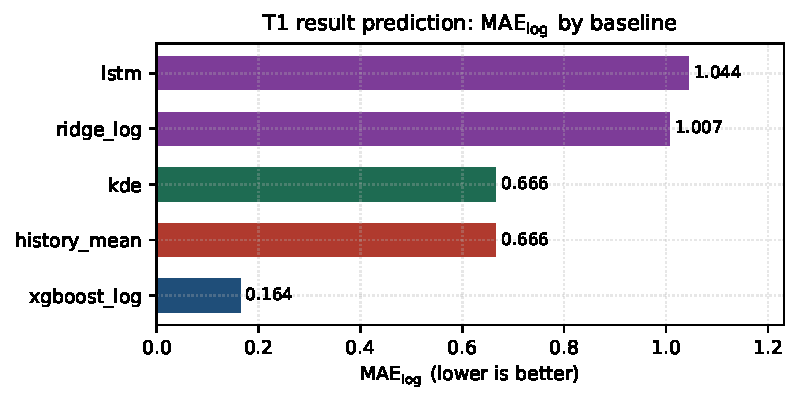
\includegraphics[width=\linewidth]{figures/fig2_result_prediction.pdf}
    \caption{\task{1} \maelog{}.}
    \label{fig:t1}
  \end{subfigure}\hfill
  \begin{subfigure}[b]{0.32\linewidth}
    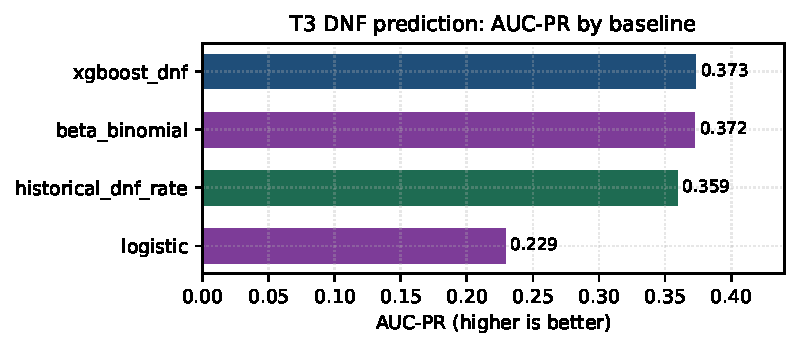
\includegraphics[width=\linewidth]{figures/fig3_dnf_models.pdf}
    \caption{\task{3} \aucpr{}.}
    \label{fig:t3}
  \end{subfigure}\hfill
  \begin{subfigure}[b]{0.32\linewidth}
    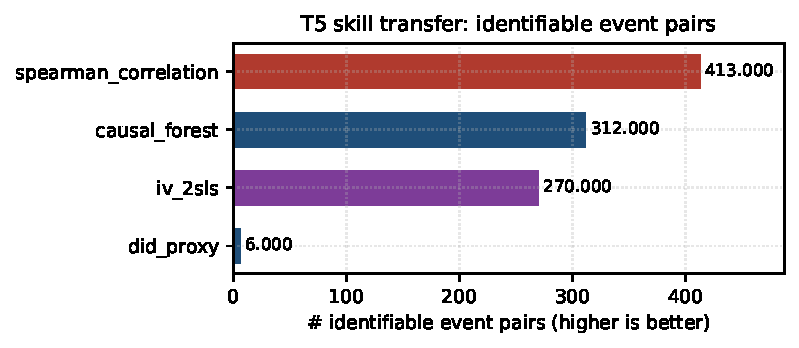
\includegraphics[width=\linewidth]{figures/fig4_transfer_pairs.pdf}
    \caption{\task{5} pairs.}
    \label{fig:t5}
  \end{subfigure}
  \caption{Per-task detail for \task{1}, \task{3} and \task{5}.}
  \label{fig:taskdetail}
\end{figure}

\subsection{Reproducing these numbers}
\label{sec:results-repro}

All numbers above are regenerated by the released pipeline:
\begin{center}\small
\code{build\_dataset} $\to$
\code{run\_all\_baselines --mode small --device cuda} $\to$
\code{run\_multi\_seed --seeds 42 43 44 --mode small --device cuda} $\to$
\code{build\_leaderboard}.
\end{center}
The offline path substitutes a synthetic generator so that continuous
integration runs without network access; results computed on synthetic data are
labelled as such and never enter the leaderboard. Each baseline writes a
structured report containing overall metrics, the four stratified views,
calibration, significance tests against the registered reference baselines and
a cost file (with device and GPU/CPU hours), exactly as specified in
Section~\ref{sec:protocol}.
